% Options for packages loaded elsewhere
\PassOptionsToPackage{unicode}{hyperref}
\PassOptionsToPackage{hyphens}{url}
\PassOptionsToPackage{dvipsnames,svgnames,x11names}{xcolor}
%
\documentclass[
  letterpaper,
  DIV=11,
  numbers=noendperiod]{scrartcl}

\usepackage{amsmath,amssymb}
\usepackage{lmodern}
\usepackage{iftex}
\ifPDFTeX
  \usepackage[T1]{fontenc}
  \usepackage[utf8]{inputenc}
  \usepackage{textcomp} % provide euro and other symbols
\else % if luatex or xetex
  \usepackage{unicode-math}
  \defaultfontfeatures{Scale=MatchLowercase}
  \defaultfontfeatures[\rmfamily]{Ligatures=TeX,Scale=1}
\fi
% Use upquote if available, for straight quotes in verbatim environments
\IfFileExists{upquote.sty}{\usepackage{upquote}}{}
\IfFileExists{microtype.sty}{% use microtype if available
  \usepackage[]{microtype}
  \UseMicrotypeSet[protrusion]{basicmath} % disable protrusion for tt fonts
}{}
\makeatletter
\@ifundefined{KOMAClassName}{% if non-KOMA class
  \IfFileExists{parskip.sty}{%
    \usepackage{parskip}
  }{% else
    \setlength{\parindent}{0pt}
    \setlength{\parskip}{6pt plus 2pt minus 1pt}}
}{% if KOMA class
  \KOMAoptions{parskip=half}}
\makeatother
\usepackage{xcolor}
\setlength{\emergencystretch}{3em} % prevent overfull lines
\setcounter{secnumdepth}{5}
% Make \paragraph and \subparagraph free-standing
\ifx\paragraph\undefined\else
  \let\oldparagraph\paragraph
  \renewcommand{\paragraph}[1]{\oldparagraph{#1}\mbox{}}
\fi
\ifx\subparagraph\undefined\else
  \let\oldsubparagraph\subparagraph
  \renewcommand{\subparagraph}[1]{\oldsubparagraph{#1}\mbox{}}
\fi


\providecommand{\tightlist}{%
  \setlength{\itemsep}{0pt}\setlength{\parskip}{0pt}}\usepackage{longtable,booktabs,array}
\usepackage{calc} % for calculating minipage widths
% Correct order of tables after \paragraph or \subparagraph
\usepackage{etoolbox}
\makeatletter
\patchcmd\longtable{\par}{\if@noskipsec\mbox{}\fi\par}{}{}
\makeatother
% Allow footnotes in longtable head/foot
\IfFileExists{footnotehyper.sty}{\usepackage{footnotehyper}}{\usepackage{footnote}}
\makesavenoteenv{longtable}
\usepackage{graphicx}
\makeatletter
\def\maxwidth{\ifdim\Gin@nat@width>\linewidth\linewidth\else\Gin@nat@width\fi}
\def\maxheight{\ifdim\Gin@nat@height>\textheight\textheight\else\Gin@nat@height\fi}
\makeatother
% Scale images if necessary, so that they will not overflow the page
% margins by default, and it is still possible to overwrite the defaults
% using explicit options in \includegraphics[width, height, ...]{}
\setkeys{Gin}{width=\maxwidth,height=\maxheight,keepaspectratio}
% Set default figure placement to htbp
\makeatletter
\def\fps@figure{htbp}
\makeatother
\newlength{\cslhangindent}
\setlength{\cslhangindent}{1.5em}
\newlength{\csllabelwidth}
\setlength{\csllabelwidth}{3em}
\newlength{\cslentryspacingunit} % times entry-spacing
\setlength{\cslentryspacingunit}{\parskip}
\newenvironment{CSLReferences}[2] % #1 hanging-ident, #2 entry spacing
 {% don't indent paragraphs
  \setlength{\parindent}{0pt}
  % turn on hanging indent if param 1 is 1
  \ifodd #1
  \let\oldpar\par
  \def\par{\hangindent=\cslhangindent\oldpar}
  \fi
  % set entry spacing
  \setlength{\parskip}{#2\cslentryspacingunit}
 }%
 {}
\usepackage{calc}
\newcommand{\CSLBlock}[1]{#1\hfill\break}
\newcommand{\CSLLeftMargin}[1]{\parbox[t]{\csllabelwidth}{#1}}
\newcommand{\CSLRightInline}[1]{\parbox[t]{\linewidth - \csllabelwidth}{#1}\break}
\newcommand{\CSLIndent}[1]{\hspace{\cslhangindent}#1}

\KOMAoption{captions}{tableheading}
\makeatletter
\makeatother
\makeatletter
\makeatother
\makeatletter
\@ifpackageloaded{caption}{}{\usepackage{caption}}
\AtBeginDocument{%
\ifdefined\contentsname
  \renewcommand*\contentsname{Table of contents}
\else
  \newcommand\contentsname{Table of contents}
\fi
\ifdefined\listfigurename
  \renewcommand*\listfigurename{List of Figures}
\else
  \newcommand\listfigurename{List of Figures}
\fi
\ifdefined\listtablename
  \renewcommand*\listtablename{List of Tables}
\else
  \newcommand\listtablename{List of Tables}
\fi
\ifdefined\figurename
  \renewcommand*\figurename{Figure}
\else
  \newcommand\figurename{Figure}
\fi
\ifdefined\tablename
  \renewcommand*\tablename{Table}
\else
  \newcommand\tablename{Table}
\fi
}
\@ifpackageloaded{float}{}{\usepackage{float}}
\floatstyle{ruled}
\@ifundefined{c@chapter}{\newfloat{codelisting}{h}{lop}}{\newfloat{codelisting}{h}{lop}[chapter]}
\floatname{codelisting}{Listing}
\newcommand*\listoflistings{\listof{codelisting}{List of Listings}}
\makeatother
\makeatletter
\@ifpackageloaded{caption}{}{\usepackage{caption}}
\@ifpackageloaded{subcaption}{}{\usepackage{subcaption}}
\makeatother
\makeatletter
\@ifpackageloaded{tcolorbox}{}{\usepackage[many]{tcolorbox}}
\makeatother
\makeatletter
\@ifundefined{shadecolor}{\definecolor{shadecolor}{rgb}{.97, .97, .97}}
\makeatother
\makeatletter
\makeatother
\ifLuaTeX
  \usepackage{selnolig}  % disable illegal ligatures
\fi
\IfFileExists{bookmark.sty}{\usepackage{bookmark}}{\usepackage{hyperref}}
\IfFileExists{xurl.sty}{\usepackage{xurl}}{} % add URL line breaks if available
\urlstyle{same} % disable monospaced font for URLs
\hypersetup{
  pdftitle={Preface},
  pdfauthor={Michael Betancourt},
  colorlinks=true,
  linkcolor={blue},
  filecolor={Maroon},
  citecolor={Blue},
  urlcolor={Blue},
  pdfcreator={LaTeX via pandoc}}

\title{Preface}
\author{Michael Betancourt}
\date{February 2023}

\begin{document}
\maketitle
\ifdefined\Shaded\renewenvironment{Shaded}{\begin{tcolorbox}[borderline west={3pt}{0pt}{shadecolor}, enhanced, frame hidden, breakable, sharp corners, boxrule=0pt, interior hidden]}{\end{tcolorbox}}\fi

\renewcommand*\contentsname{Table of contents}
{
\hypersetup{linkcolor=}
\setcounter{tocdepth}{3}
\tableofcontents
}
Common experience tells us that unsupported objects fall towards the
ground under the influence of Earth's gravity. To understand this
phenomenon more \emph{quantitatively} we need to compare observations of
falling objects to mathematical models, each capturing a distinct story
of how objects fall. In particular we might carefully observe the
trajectory that a ball traces out after it is released and then compare
those observations to different mathematical models for that motion
given the ball's initial height and velocity and the local acceleration
due to gravity.

If the measurements were infinitely precise
(Figure~\ref{fig-exact-data}) then we would be able to exclude any model
that doesn't \emph{exactly} reproduce the observed trajectory
(Figure~\ref{fig-exact-fit}).

\begin{figure}

\begin{minipage}[t]{0.50\linewidth}

{\centering 

\raisebox{-\height}{

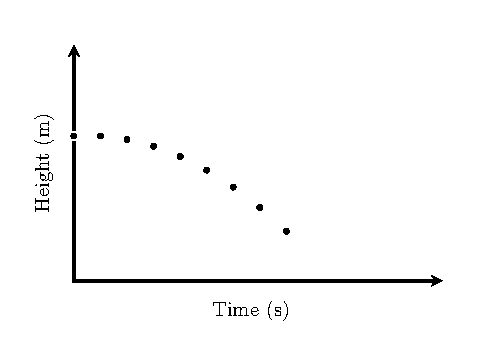
\includegraphics{figures/gravity/exact_data/exact_data.pdf}

}

}

\subcaption{\label{fig-exact-data}}
\end{minipage}%
%
\begin{minipage}[t]{0.50\linewidth}

{\centering 

\raisebox{-\height}{

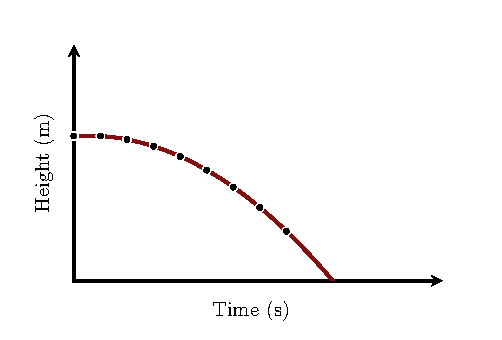
\includegraphics{figures/gravity/exact_fit/exact_fit.pdf}

}

}

\subcaption{\label{fig-exact-fit}}
\end{minipage}%

\caption{\label{fig-ideal}In an ideal world (a) infinitely precise
observations of a falling ball (b) would exclude all mathematical models
of gravity except for those that exactly reproduce the observations.}

\end{figure}

Unfortunately even the most skilled scientist cannot achieve infinitely
precise measurements. Practical measurements of a falling object are
limited not only by chaotic atmospheric forces imparted on the ball as
it falls but also finite spatial resolution. Even if we knew the true
model we still would not be able to exactly predict the outcome of each
measurement (Figure~\ref{fig-realistic-data}).

\begin{figure}

{\centering 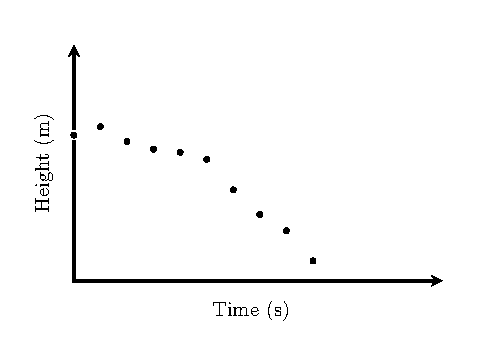
\includegraphics[width=0.5\textwidth,height=\textheight]{figures/gravity/data/data.pdf}

}

\caption{\label{fig-realistic-data}Realistic measurements are
unpredictable, at best scattering around the true model.}

\end{figure}

Without precise predictability we cannot exclude most models outright;
just about every model will perfectly reproductive a given observation
with a sufficiently convenient fluctuation in the measurement. Even if
we can restrict consideration to \emph{typical} fluctuations many
different gravitational models will be consistent with the observed data
(Figure~\ref{fig-consistent-configs}).

\begin{figure}

\begin{minipage}[t]{0.50\linewidth}

{\centering 

\raisebox{-\height}{

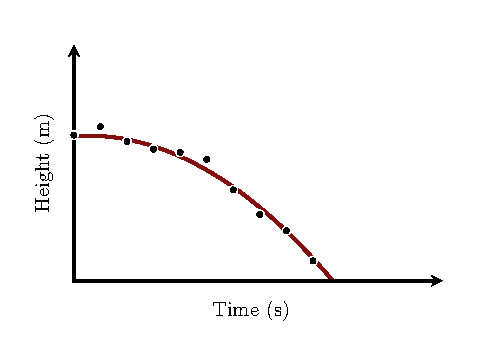
\includegraphics{figures/gravity/data_consistent_config1/data_consistent_config1.pdf}

}

}

\subcaption{\label{fig-consistent-config1}}
\end{minipage}%
%
\begin{minipage}[t]{0.50\linewidth}

{\centering 

\raisebox{-\height}{

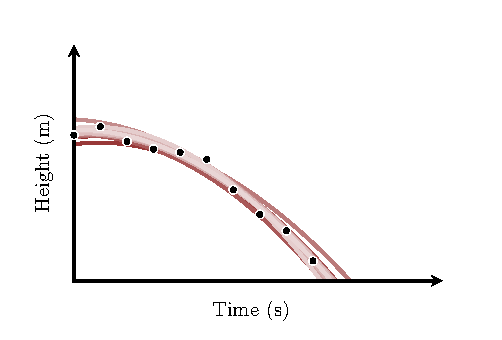
\includegraphics{figures/gravity/data_consistent_config3/data_consistent_config3.pdf}

}

}

\subcaption{\label{fig-consistent-config3}}
\end{minipage}%

\caption{\label{fig-consistent-configs}The lack of predictability in
practical measurements complicates learning from data. (a) Every model
that is consistent with a noisy observation is accompanied by (b) many
other models that are similarly consistent.}

\end{figure}

In other words any inferences we can draw from a realistic observation
will be fundamentally \emph{uncertain}. If we want to extract robust
insights from data we have to face this uncertainty.

Consider, for example, learning about the environment around us through
experiment and observation, either for pure curiosity or to inform
particular decisions about how to interact with that environment. The
\textbf{scientific method} organizes this learning process into a
systematic procedure (Figure~\ref{fig-scientific-method-nominal}).

\begin{figure}

{\centering 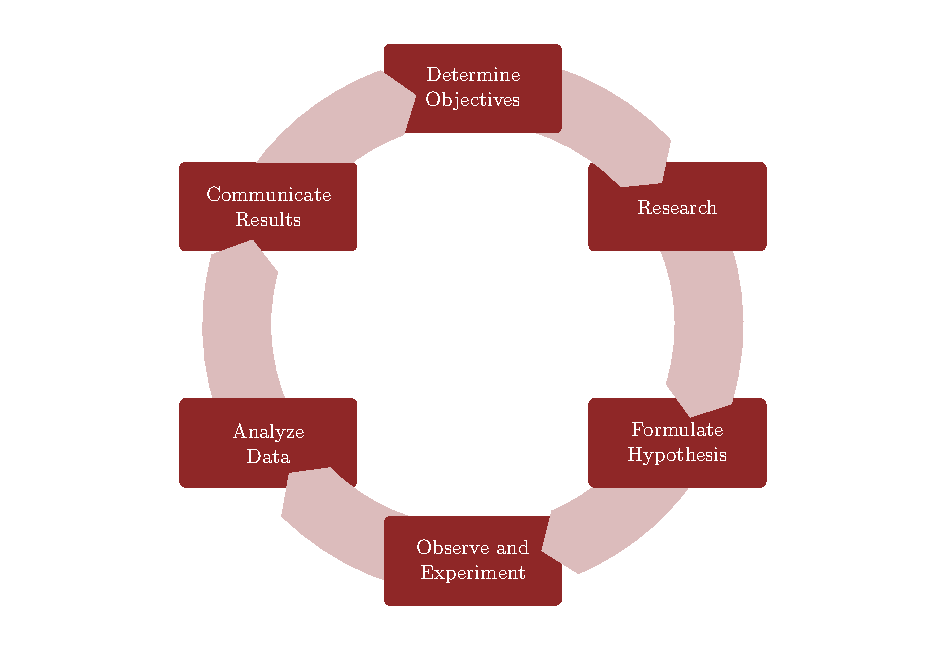
\includegraphics[width=0.75\textwidth,height=\textheight]{figures/scientific_method/nominal/nominal.pdf}

}

\caption{\label{fig-scientific-method-nominal}The scientific method
reduces the process of learning from experiment and observation into a
sequence of basic steps, including one where we have to draw inferences
from observed data.}

\end{figure}

While the basic steps of this procedure might appear straightforward,
the complexity of scientific inquiry is hidden in the details of their
implementation. In particular when trying to implement the ``Analyze
Data'' step we have to confront the fundamental limitations measurements
and determine how to quantify our inferential uncertainty. Formally
quantifying inferential uncertainty is exactly the goal of
\textbf{statistical inference}.

To realize the ``Analyze Data'' step, and hence the scientific method as
a whole, we have to encode our knowledge into mathematical models,
identify how consistent those models are with a given observation, and
then verify that the consistent models adequately reproduce the
structure of that observation (Figure~\ref{fig-scientific-method-box}).
As George Box noted we cannot do rigorous science without rigorous
statistical modeling and inference (Box 1976).

\begin{figure}

{\centering 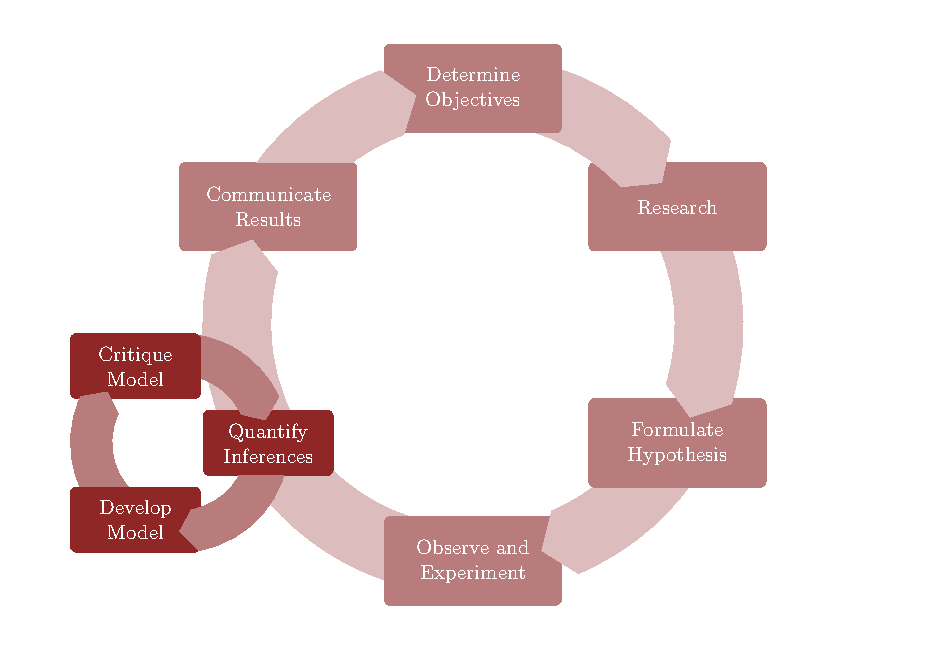
\includegraphics[width=0.75\textwidth,height=\textheight]{figures/scientific_method/box/box.pdf}

}

\caption{\label{fig-scientific-method-box}Each step in the scientific
method encapsulates many critical implementation details. For example in
order to ``Analyze Data'' we need to be able to develop candidate
mathematical models, each representing one way that observations could
be generated, and then quantifying how consistent each of those models
are with an actual observation.}

\end{figure}

In this book we will learn how to use \textbf{Bayesian inference} to
analyze data and, ultimately, implement the scientific method for both
scientific and industrial applications. Bayesian inference uses
\textbf{probability theory} to not only develop \textbf{probabilistic
models} of measurements but also to quantify how consistent those models
are with our domain expertise and observed data
(Figure~\ref{fig-bayesian-configs})

\begin{figure}

\begin{minipage}[t]{0.50\linewidth}

{\centering 

\raisebox{-\height}{

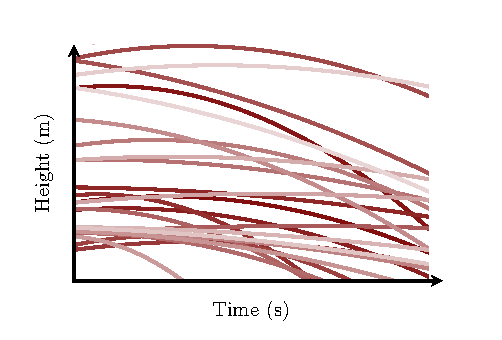
\includegraphics{figures/gravity/prior_ensemble/prior_ensemble.pdf}

}

}

\subcaption{\label{fig-config_prior}}
\end{minipage}%
%
\begin{minipage}[t]{0.50\linewidth}

{\centering 

\raisebox{-\height}{

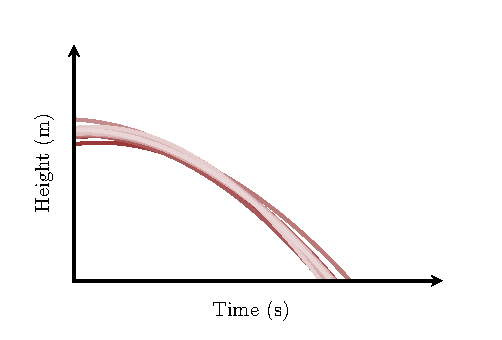
\includegraphics{figures/gravity/posterior_ensemble/posterior_ensemble.pdf}

}

}

\subcaption{\label{fig-config-posterior}}
\end{minipage}%

\caption{\label{fig-bayesian-configs}Bayesian inference uses probability
theory to quantify which models (a) how a priori consistent models are
with any available domain expertise and then (b) how a posteriori
consistent they are with both the available domain expertise and any
observed data.}

\end{figure}

Although Bayesian inference is conceptually elegant its practical
implementation is far from trivial. In order to implement a successful
Bayesian analysis we need be proficient with not only building models
but also critiquing their adequacy in a particular application and
accurately quantify their consistency with observed data. This books
considers not only the conceptual foundations of Bayesian inference but
also these implementation challenges so that by its conclusion you will
be prepared to build the \emph{bespoke} analysis unique to your
particular application.

\hypertarget{the-pedagogical-approach-of-this-book}{%
\section{The Pedagogical Approach Of This
Book}\label{the-pedagogical-approach-of-this-book}}

To execute such an ambitious goal as painlessly as possible we need a
careful \emph{pedagogical} strategy. What is the best way to learn how
to robustly implement Bayesian analyses?

In this section I'll discuss what I think is the best way to learn
Bayesian inference and hence why this book is structured so differently
from many other introductions to Bayesian analysis.

\hypertarget{abstractions}{%
\subsection{Abstractions}\label{abstractions}}

Most subjects, including Bayesian inference are conceptually dense.
While they might superficially appear simple the more closely we examine
them the more detail we need to confront in order to form a coherent
theory. In order to make a subject approachable for students we have to
rely on pedagogical \textbf{abstractions} that hide the overwhelming
depth behind only a selection of concepts that are easier to digest.

A good abstraction focuses on simple concepts that are mostly consistent
with each other. This consistency keeps the abstraction largely
self-contained, obscures the hidden depth below. Scrutinizing the
inconsistencies that do manifest in a given abstraction, however, will
eventually lead us beyond the boundaries of that abstraction and into
the domain of a new, deeper abstraction. When developing practical
methodologies we need to find a sufficiently rich abstraction that
captures all of the necessary concepts without too much unnecessary
detail.

Consider, for example, the real numbers. At a high-level we can
conceptualize the real numbers as a \emph{continuum} with infinite
detail no matter how closely we zoom in. This is a completely reasonable
abstraction for most applications involving not only basic arithmetic
but also more complicated operations like differentiation and
integration. When we want to engage in more technical results, however,
we will need to go beyond this simple abstraction in order to develop a
consistent theory free of pathological behavior.

Abstractions also play a role in how real numbers are implemented in
practice. At a high-level we can assume that computers are able to
exactly represent real numbers and exactly implement their arithmetic
operations. In many applications this abstraction is entirely valid.
When working on applications that require precise or complicated
calculations, however, we start to see cracks in this conceptual
picture.

Eventually we have to confront the reality of the \emph{finite precision
arithmetic} implemented on computers and how it deviates from exact
arithmetic. Going slightly deeper we might consider the limited dynamic
range of \emph{floating point} numbers that can result in underflow and
overflow for particularly small and large results. Digging even further
we might tackle how underflow and overflow in intermediate calculations
can lead to catastrophic errors even if the final result is not itself
extremely small or large.

\hypertarget{sequences-of-abstractions}{%
\subsection{Sequences of Abstractions}\label{sequences-of-abstractions}}

In most applications an abstraction that is sufficiently detailed is too
overwhelming to approach all at once. Instead we have to progress
towards it carefully through a sequence of intermediate abstractions.
This leaves us to consider the progressions that best guide students
towards that terminal abstraction.

\hypertarget{non-overlapping-progressions}{%
\subsubsection{Non-Overlapping
Progressions}\label{non-overlapping-progressions}}

One approach, for example, utilizes a progression of
\emph{non-overlapping} abstractions (Figure~\ref{fig-abs-incons}). This
allows the intermediate abstractions to incorporate compelling
intuitions and examples even if they don't generalize to the final
abstraction. Moreover each abstraction can be compartmentalized into a
relatively self-contained course, and different students with different
goals can follow the progression to different terminal abstractions. For
these reasons this approach is particularly common in academia.

\begin{figure}

\begin{minipage}[t]{0.33\linewidth}

{\centering 

\raisebox{-\height}{

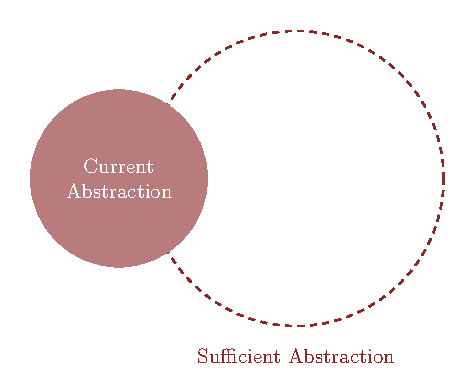
\includegraphics{figures/pedagogical_abstractions/inconsistent/1/1.pdf}

}

}

\subcaption{\label{fig-abs-incons1}}
\end{minipage}%
%
\begin{minipage}[t]{0.33\linewidth}

{\centering 

\raisebox{-\height}{

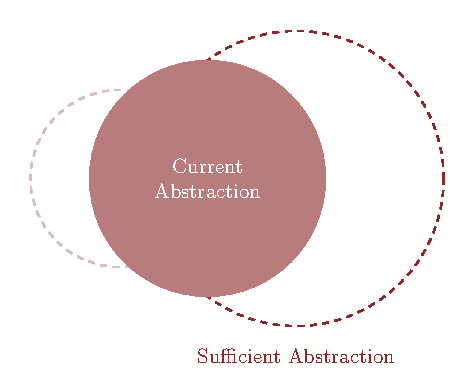
\includegraphics{figures/pedagogical_abstractions/inconsistent/2/2.pdf}

}

}

\subcaption{\label{fig-abs-incons2}}
\end{minipage}%
%
\begin{minipage}[t]{0.33\linewidth}

{\centering 

\raisebox{-\height}{

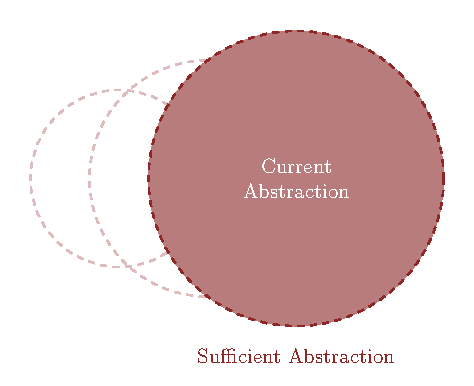
\includegraphics{figures/pedagogical_abstractions/inconsistent/3/3.pdf}

}

}

\subcaption{\label{fig-abs-incons3}}
\end{minipage}%

\caption{\label{fig-abs-incons}Non-overlapping progressions build up to
a final, sufficient abstraction through inconsistent intermediate
abstractions. At each iteration only some of the concepts are carried
forward to the new, more detailed abstraction.}

\end{figure}

Non-overlapping progressions can be problematic, however, when the
sequence of intermediate abstractions terminates prematurely. The
insights of the last intermediate abstraction encountered might be
useful in some circumstances, but without the context of the remaining
abstractions a student will likely have difficulty identifying exactly
what those necessary circumstances, let alone validating when they hold
in a given application. In other words the understanding offered by only
an intermediate abstraction can be \emph{fragile} when the assumptions
holding that abstraction together cannot be taken for granted.

Another problem with this approach is that the updating from one
abstraction to the next can be burdensome on students. Because the
abstractions don't overlap a student doesn't just expand their
understanding with new concepts at each iteration; instead they also
have to \emph{unlearn} the concepts that don't generalize from the
previous abstraction (Figure~\ref{fig-unlearning}). This repeated cycle
of learning and unlearning can be frustrating and even discourage
students from moving past an intermediate, and potentially fragile,
abstraction.

\begin{figure}

\begin{minipage}[t]{0.33\linewidth}

{\centering 

~

}

\end{minipage}%
%
\begin{minipage}[t]{0.33\linewidth}

{\centering 

\raisebox{-\height}{

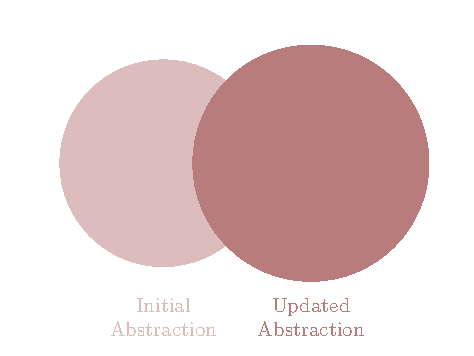
\includegraphics{figures/pedagogical_abstractions/unlearning/1/1.pdf}

}

}

\subcaption{\label{fig-unlearning1}}
\end{minipage}%
%
\begin{minipage}[t]{0.33\linewidth}

{\centering 

~

}

\end{minipage}%
\newline
\begin{minipage}[t]{0.33\linewidth}

{\centering 

\raisebox{-\height}{

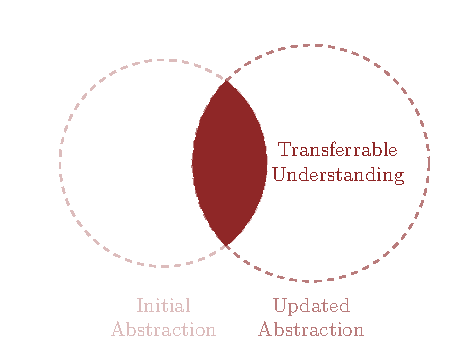
\includegraphics{figures/pedagogical_abstractions/unlearning/2/2.pdf}

}

}

\subcaption{\label{fig-unlearning2}}
\end{minipage}%
%
\begin{minipage}[t]{0.33\linewidth}

{\centering 

\raisebox{-\height}{

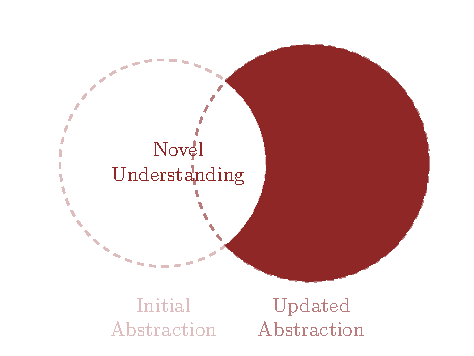
\includegraphics{figures/pedagogical_abstractions/unlearning/3/3.pdf}

}

}

\subcaption{\label{fig-unlearning3}}
\end{minipage}%
%
\begin{minipage}[t]{0.33\linewidth}

{\centering 

\raisebox{-\height}{

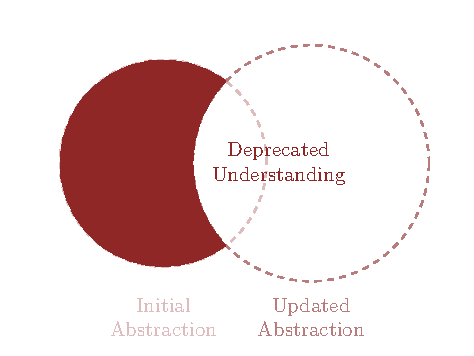
\includegraphics{figures/pedagogical_abstractions/unlearning/4/4.pdf}

}

}

\subcaption{\label{fig-unlearning4}}
\end{minipage}%

\caption{\label{fig-unlearning}The (a) inconsistent abstractions in a
non-overlapping progression can frustrate learning. At each iteration
(b) only some concepts will generalize and transfer from one abstraction
to the next and (c) the newer abstraction will also introduce new
concepts that have to be learned. (d) Some concepts in the initial
abstraction, however, will not generalize. Students have to actively
\emph{unlearn} these concepts in order to fully grasp the newer
abstraction.}

\end{figure}

For example a non-overlapping approach towards teaching arithmetic on
computers might start by assuming that computers implement arithmetic
exactly. In this case the initial abstraction can demonstrate
implementation with simple programs that define real variables and
evaluate arithmetic operations with negligible error. Students can then
use these initial insights to write new programs that can yield
reasonable results in many cases but might exhibit large, often ignored
errors in others. A following abstraction might introduce programs that
explicitly demonstrate errors before introducing the practical reasons
why real numbers and their basic operations can't be exactly implemented
on computers with finite resources. The progression could then continue
to abstractions that introduce the basic structure of fixed-point and
floating-point arithmetic and their pitfalls before presenting the
technical details of fixed-point and floating-point arithmetic
implementations on contemporary computers.

\hypertarget{overlapping-progressions}{%
\subsubsection{Overlapping
Progressions}\label{overlapping-progressions}}

Alternatively we can build up to that final, sufficient abstraction with
a progression of \emph{overlapping} abstractions
(Figure~\ref{fig-abs-cons}). By avoiding concepts that don't persist to
the final abstraction entirely nothing has to be unlearned, and students
can instead focus on expanding their understanding to the new concepts
introduced at each iteration.

\begin{figure}

\begin{minipage}[t]{0.33\linewidth}

{\centering 

\raisebox{-\height}{

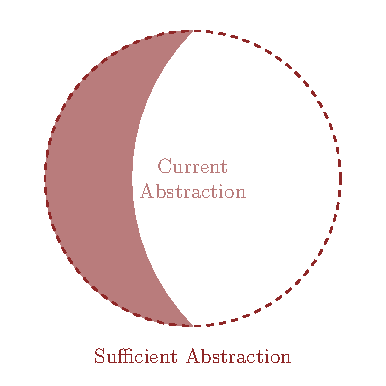
\includegraphics{figures/pedagogical_abstractions/consistent/1/1.pdf}

}

}

\subcaption{\label{fig-abs-cons1}}
\end{minipage}%
%
\begin{minipage}[t]{0.33\linewidth}

{\centering 

\raisebox{-\height}{

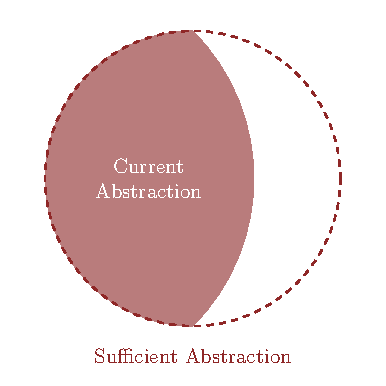
\includegraphics{figures/pedagogical_abstractions/consistent/2/2.pdf}

}

}

\subcaption{\label{fig-abs-cons2}}
\end{minipage}%
%
\begin{minipage}[t]{0.33\linewidth}

{\centering 

\raisebox{-\height}{

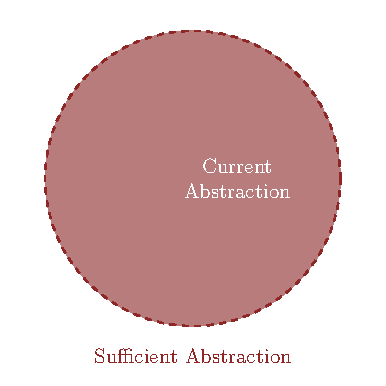
\includegraphics{figures/pedagogical_abstractions/consistent/3/3.pdf}

}

}

\subcaption{\label{fig-abs-cons3}}
\end{minipage}%

\caption{\label{fig-abs-cons}Overlapping progressions build up to a
final, sufficient abstraction through consistent intermediate
abstractions. At each iteration all of the concepts are carried forward
to the new, more detailed abstraction avoiding any need to unlearn
deprecated concepts.}

\end{figure}

Unfortunately the concepts that don't generalize often provide more
explicit, compelling motivation than the concepts that do generalize.
Because of this intermediate abstractions along an overlapping
progression can be difficult to relate to the ultimate objectives. At
the same time the persistent concepts alone, and hence the intermediate
abstractions they shape, often appear incomplete, at least until the
progression approaches the final abstraction. Consequently to benefit
from a non-overlapping approach students have to be sufficiently
dedicated to persevere through the early, less concrete abstractions.

For example an overlapping approach to teaching computer arithmetic
might start not with any demonstrative code but rather a discussion of
the infinite memory it would take to store an arbitrary real number, the
infinite processing power it would take to evaluate arithmetic for
arbitrary real numbers. A subsequent abstraction might consider the
various ways that we can theoretically approximate real numbers and
their operations with only finite memory and finite processing power.
Without explicit implementations, and code demonstrating those
implementations, there is nothing that students can abuse but also
nothing with which students can experiment and build their
comprehension. Only in later abstractions where we see how
finite-precision arithmetic is implemented will we be able to construct
interactive examples.

\hypertarget{why-this-book-is-so-long}{%
\subsection{Why This Book Is So Long}\label{why-this-book-is-so-long}}

I think that it's fair to say that most pedagogical resources take a
non-overlapping approach to teaching statistics in general, let alone
Bayesian inference in particular. In order to reach demonstrative
examples as soon as possible these resources typically begin with simple
models and little if any critique of the assumptions implied by those
models. At the same time the construction of inferences from these
models is often delegated to tools whose accuracy is taken for granted.
Few resources move beyond these relatively shallow abstractions leaving
students unaware at how fragile some of the insights might be.

Many of these resources inspire enthusiasm for Bayesian inference which,
and I mean this sincerely, cannot be discounted. Enthusiasm alone,
however, may not be enough for students to avoid the consequences of
fragile insights. Many students struggle to connect the simple models of
shallow abstractions to their own applications. Some identify the
problematic consequences of applying simple models when they're not
appropriate but, without a broader context, mistakenly blame their own
implementation of those models and not the models themselves.

This book is for those students. I embrace an overlapping progression to
deliberately, if slowly, develop the probabilistic tools needed to build
\emph{bespoke} models appropriate to a particular application and
implement \emph{faithful} Bayesian inference that accurately quantifies
uncertainty for those models. Our goal is artisanal models, not
something mass produced and sold at big box stores.

Depending on your previous experience with probabilistic modeling and
Bayesian inference you may find useful insights by jumping straight into
later chapters. That said this book is designed to be read from
beginning to end as concepts, terminology, and mathematical notation are
all built up progressively from the beginning. Starting from the
beginning will also help you confront and unlearn any misconceptions
about probability, modeling, and inference that you may have picked up
along your journey.

I do not assume any prior knowledge of the theory or practical
implementation of probability theory, probabilistic modeling, or
Bayesian inference, but I do assume some basic mathematical experience.
In particular the book will require a conceptual understanding of
calculus, namely the basic theory and implementation of differentiation
and integration, as well as working knowledge of linear algebra.

Most introductory calculus textbooks, such as Larson, Hostetler, and
Edwards (2005) and Stewart (2015), will cover the relevant concepts.
More sophisticated treatments like Apostol (1967) and Apostol (1969)
aren't necessary but can be helpful references when looking into some
more subtle technical details. For linear algebra Trefethen and Bau
(1997) is particularly thorough about not just the basic of linear
algebra but also the common pitfalls of its practical implementation.

Later chapters introduce code demonstrations in \texttt{R} and
\texttt{Python}. If you are comfortable with either language then I
encourage you to not just look through the code but also run it
yourself. Playing around with these code demonstrations is a powerful
way to develop and reinforce your comprehension.

The Carpentries offer a
\href{https://carpentries.org/workshops-curricula/\#swc-all}{variety of
workshops} that introduce both \texttt{R} and \texttt{Python}. Jenny
Bryant's \href{https://stat545.com}{Stat545 course material} is another
great resource for introducing oneself to \texttt{R} and Sweigart (2019)
is a nice resource for learning \texttt{Python}.

\hypertarget{outline}{%
\section{Outline}\label{outline}}

With all of that said let's look at the pedagogical progression of this
book in a bit more detail. The book it organized into three parts: the
first focuses on applied probability theory, the second on the general
principles of probabilistic modeling and statistical inference, and the
third on particular modeling techniques.

In Part I we will learn the mathematical properties of probability
distributions, the operations that we can use to manipulate probability
distributions, and some of the most useful methods for approximately
implementing those operations in practice. The first few chapters will
necessarily be a bit abstract until we can properly set up those
implementations but your patience will be rewarded. Overall these
chapter will go into much more detail about probability theory than most
introductions to Bayesian inference, although that that detail will
focus on conceptual understanding and practical insights rather than
technical formalities and proofs.

A thorough understanding of applied probability theory sets the stage
for Part II where we will use probability distributions to quantify
unpredictable measurements in theory, approximately model the processes
which give rise to measurements in practice, and quantify our
uncertainty about how consistent various approximations are with the
outcome of a specific measurement. In particular we will focus on
techniques to translate our understanding of a system and measurements
that interrogate that system into bespoke probabilistic models capable
to gleaming precise insights from data.

With that conceptual foundation established Part III considers
particular modeling techniques that can be useful as modular building
blocks for developing these bespoke models. Each chapter focuses on not
only the assumptions inherit to a given technique and how to validate
those assumptions but also on efficient implementations. Many of the
chapters will consider popular estimation techniques from the modeling
perspective we need to rigorously integrate them into Bayesian analyses.

Although Part III introduces many modeling techniques it is by no means
exhaustive. One of the exciting aspects of probabilistic modeling is an
eternal opportunity to learn new techniques, expanding our modeling
toolkit and the sophistication of bespoke models that we can employ in
practice. This book will hopefully prepare you for that never-ending,
but never-boring journey.

\hypertarget{license}{%
\section*{License}\label{license}}
\addcontentsline{toc}{section}{License}

A repository containing all of the files used to generate this chapter
is available on
\href{https://github.com/betanalpha/quarto_chapters/tree/main/preface}{GitHub}.

The text and figures in this chapter are copyrighted by Michael
Betancourt and licensed under the CC BY-NC 4.0 license:

https://creativecommons.org/licenses/by-nc/4.0/

\hypertarget{refs}{}
\begin{CSLReferences}{1}{0}
\leavevmode\vadjust pre{\hypertarget{ref-Apostol:1967}{}}%
Apostol, Tom M. 1967. \emph{Calculus. {V}ol. {I}: {O}ne-Variable
Calculus, with an Introduction to Linear Algebra}. Second. Blaisdell
Publishing Co. {[}Ginn; Co.{]}, Waltham, Mass.-Toronto, Ont.-London.

\leavevmode\vadjust pre{\hypertarget{ref-Apostol:1969}{}}%
---------. 1969. \emph{Calculus. {V}ol. {II}: {M}ulti-Variable Calculus
and Linear Algebra, with Applications to Differential Equations and
Probability}. Second. Blaisdell Publishing Co. {[}Ginn; Co.{]}, Waltham,
Mass.-Toronto, Ont.-London.

\leavevmode\vadjust pre{\hypertarget{ref-Box:1976}{}}%
Box, George E. P. 1976. {``Science and Statistics.''} \emph{J. Amer.
Statist. Assoc.} 71 (356): 791--99.

\leavevmode\vadjust pre{\hypertarget{ref-LarsonEtAl:2005}{}}%
Larson, R., R. P. Hostetler, and B. H. Edwards. 2005. \emph{Calculus of
a Single Variable}. Houghton Mifflin College Division.

\leavevmode\vadjust pre{\hypertarget{ref-Stewart:2015}{}}%
Stewart, J. 2015. \emph{Calculus}. 8th ed. Cengage Learning.

\leavevmode\vadjust pre{\hypertarget{ref-Sweigart:2019}{}}%
Sweigart, Al. 2019. \emph{Automate the Boring Stuff with Python:
Practical Programming for Total Beginners}. No Starch Press.

\leavevmode\vadjust pre{\hypertarget{ref-TrefethenEtAl:1997}{}}%
Trefethen, Lloyd N., and David Bau III. 1997. \emph{Numerical Linear
Algebra}. Society for Industrial; Applied Mathematics (SIAM),
Philadelphia, PA.

\end{CSLReferences}



\end{document}
